% !TEX root = 00_arbeit.tex

%---------------------------------------------------------------------------------
%% Literaturrecherche

\section{Aktuelle Preismodellierung auf Strommärkten}\label{sec:strompreis}

\todo{Kapitel einleiten}

\subsection{Der Strommarkt und seine Vorhersagemodelle}\label{sec:vorhersagemodelle}

Elektrizität ist eine besonderes Gut, dessen Erzeugung und Verbrauch gleichzeitig erfolgt. Die Erzeugung dieses Gutes kann kontrolliert werden. Wobei sich das Speichern von Elektrizität in einem industriellen Maßstab als schwierig gestaltet. Daher beeinflusst die Nachfrage maßgeblich die zu generierende Menge. Aus diesem Grund verläuft der Handel, im Gegensatz zu anderen Finanz- oder Gütermärkten, oft auf dem sogenannten „Day-ahead“-Markt. Der Strom wird dabei für jede Stunde des nächsten Tages ge- und verkauft. Diese Handelsweise ist für die Marktakteure notwendig, um die Produktions- und Abnahmekapazitäten einander anzupassen. Auf den meisten Märkten müssen die Marktakteure bis zu einer bestimmten Frist ihre 24 Gebote abgeben. Nach Ablauf der Frist erstellt der Marktbetereiber, unter Berücksichtigung aller Gebote, den Gleichgewichtspreis (engl.: market clearing price) für jede der 24 Stunden. Produzenten deren Gebot niedriger bzw. Konsumenten deren Gebot höher oder gleich dem Gleichgewichtspreis ist, bekommen den Zuschlag.\citef[7]{Weron2014} Um den Gleichgewichtspreis des nächsten Tages vorherzusagen und ein Gebot möglichst nah am Gleichgewichtspreis abzugeben, gibt es vielfältige Ansätze.

Einen guten Überblick über vorgeschlagene Modelle zur Strompreisvorhersage geben \citet{Aggarwal2009}, \citet{Cerjan2013}, \citet{Weron2014} und \citet{Panapakidis2016} in ihren Reviews. Zunächst können die in \autoref{fig:ann_vorhers._modelle} dargestellten Modelle in einen lang-/mittelfristigen und kurzfristigen Vorhersagehorizont eingeteilt werden. 

\begin{figure}[!htb]
    \centering
        \includegraphics[page=2,width=1\textwidth]{Bilder/misc/ANN_Organigramme.pdf}
    \caption{Organigramm der Modelle die zur Vorhersage des Strompreises eingesetzt werden.\protect\footnotemark{}}
    \label{fig:ann_vorhers._modelle}
\end{figure}
\addtocounter{footnote}{-1}     % -1 mal die Gesamtanzahl an Fußnoten in der wrapfigure
\addtocounter{Hfootnote}{-1}    % -1 times total number of footnote(mark)s in the wrapfigure
\wrapfigfoot\footnotetext{\autoref{fig:ann_vorhers._modelle} wurde in Anlehnung an \citet[12]{Weron2014} erstellt.}



Zu dem lang- und mittelfristigen Vorhersagehorizont kommen folgende Modelle zur Anwendung:
\begin{itemize}
\item[\textbf{$\bullet$}]%
Multi-Agenten bzw. Spieltheorie Modelle, bei denen versucht wird das Verhalten der unterschiedlichen Agenten/Akteure auf dem Markt zu simulieren.

\item[\textbf{$\bullet$}]%
Fundamentale Modelle, bei denen physikalische Faktoren in Zusammenhang mit der Preisdynamik gesetzt werden.

\item[\textbf{$\bullet$}]%
Reduzierte Modelle, welche die statistischen Eigenschaften des zeitlichen Preisverlaufes mit Hilfe der Auswertung von Risiken und Derivaten erklären.
\end{itemize}

Für den kurzfristigen Vorhersagehorizont werden die nachfolgenden Modelle angewandt:
%Zusammenfassend lassen sich die Modelle in folgende Kategorien einteilen:
%\citet{Weron2014} hat die vorgeschlagenen Modelle zur Preisvorhersage in in fünf Kategorien eingeteilt:\footnote{In der Literatur vorkommende Modelle sind oftmals hybride Lösungen, die aus mehreren der genannten Kategorien bestehen.}
\begin{itemize}
\item[\textbf{$\bullet$}]%
Statistische Modelle, welche aus linearer Regression von Zeitreihen und ökonometrischen Modellen bestehen.

\item[\textbf{$\bullet$}]%
Komputerbasierte/künstliche Intelligenz (CI), die in Verbindung mit Lern-,Evolutions- und Fuzzyalgorithmen komplexe dynamische Systeme abbilden kann.
\end{itemize}

Wobei die Modelle komputerbasierte/künstliche Intelligenz weiter unterteilt werden in: 
\begin{itemize}
\item[\textbf{$\bullet$}]%
Künstliche Neuronale Netze

\item[\textbf{$\bullet$}]%
Data-Mining Modelle
\end{itemize}

%\todo{Der Unterschied zwischen künstlichen neuronalen Netzen und Data-Mining + Modelle nennen }

Die passende Methode zur Strompreisvorhersage hängt von einer Vielzahl von Überlegungen ab. Der Frage welche Methode die Beste ist, um Vorhersagen zu treffen stellt \citet{Chatfield1988} in seiner Arbeit. Vor diesem Hintergrund stellt er sechs Empfehlungen aus. Unter anderem ist die Komplexität eines Modells kein Garant für bessere Vorhersagen im Vergleich zu weniger komplexen Modellen. Weiterhin kann die Anzahl an vergangenen Beobachtungen und der gewünschte Vorhersagehorizont eine Orientierung bei der Wahl des passenden Modells geben.
Bei ihren Untersuchungen stellen \citet{Nogales2002} fest, dass in den meisten kompetitiven Strommärkten die Zeitreihen der Strompreise eine hohen Schwankung aufweisen (gleichzusetzen mit hoher Volatilität), mehrere Sesionalitäten besitzen (das heißt, dass die Zeitreihen tages- und wochenabhängigen Peridiozitäten unterielgen ), einen Kallender-Effekt besitzen (Abhängigkeiten von Wochenenden und Feiertagen) und einen hohen prozentualen Anteil an ungewöhnlichen Preisverläufen besitzen. \citet{Vijayalakshmi2015} kommen bei ihrem Review von NN-Implementierungen für die Strompreisprognose zu dem Schluss, dass sich Strompreise, die durch Volatilität, Saisonalität, Preis-Spitzen, Sprünge und Nichtlinearitäten gekennzeichnet sind, oft nur schwer mit ökonometrischen Modellen vorhersagen lassen. NN-basierte Modelle können aber eine mögliche Antwort auf die kurzfristige Strompreisprognose sein. \citet{Weron2014} kommt zu dem Schluss, dass die Stärke der computerbasierten Intelligenz Modelle in der Fähihgkeit liegt, mit Komplexität und Nichtlinearität umgehen zu können. \citet{Gareta2006} sind jedoch der Meinung, dass Ergebnisse der NN-Modelle abhängig von der Menge der Eingabedaten sind und dass das Modell einer Überprüfung bedarf.

Die Anzahl und Einteilung der Modelle in unterschiedliche Vorhersagehorizonte weist darauf hin, dass nicht ein Modell allein alle Faktoren, die zum schließlichen Preis führen, erfasst. Aus diesem Grund werden in der Literatur hybride Modelle eingesetzt die aus einigen der genannten Kategorien zusammen gesetzt sind. \citet{Cerjan2013} begründen die Benutzung hybrider Modelle damit, dass die einzelnen Modelle unterschiedliche Muster in den Daten erfassen können. Die einzelnen Modelle ermöglichen damit eine Verringerung der Vorhersageabweichungen und verhelfen den Marktakteuren zu dem erhofften Zuschlag.


\subsection{Literaturüberblick zur Anwendung von neuronaler Netze zur Strompreisvorhersage}\label{sec:literaturueberblick}

\citet{Aggarwal2009} und \citet{Panapakidis2016} haben eine tabelarische Übersicht über die bis dato genutzten NN basierten Modelle zur Vorhersage des Elektrizitätspreises vorgestellt. In Anlehnung der beiden Veröffentlichungen erfolgt ein Literaturüberblick von Anfang 2016 bis ende 2017. 
Modelle basierend auf NN, die in dieser Zeit veröffentlicht und dem Autor dieser Arbeit zur Verfügung standen, sind in \autoref{tab:ann_lit} dargestellt. Neben den Verweisen sind die eingesetzten Netzwerke, die untersuchten Märkte und das zur Evaluation eingesetzte Performancemaß aufgeführt. In der genannten Literatur kommen zum Teil hybride Modelle vor. Da es der Fokus dieser Arbeit ist, einen Überblick über die Anwendung neuronaler Netze zur Strompreisvorhersage zu geben, wurde in der Tabelle nur das zur Anwendung kommende neuronale Netz aufgeführt. 

%\todo{Übersicht über die Märkte und Performancemaße im Anhang erstellen und im Text auf sie Verweisen}

In der betrachteten Zeitperiode werden in der Literatur zur Vorhersage von Strompreisen die verwendeten Netzwerk Modelle als Artificial neural Network (ANN) bei \citet{Mirakyan2017}, \citet{Gao2017} und \citet{Sandhu2016} aufgeführt. Wobei \citet{Davo2016} und \citet{Domanski2017} den allgemeinen Begriff neural Network (NN) nutzen. Weitere Begriffe sind Backpropagation neural Network (BPNN) bei \citet{Wang2017}, Feed-Forward neural Networks bei \citet{Keles2016} oder die Kombination aus beiden Feed-Forward Backpropagation neural Network (FFBPNN) bei \citet{Peter2016}. Zuletzt sind noch Function-Fitting neural Network (FFNN) bei \citet{Marcos2017} und Deep neural Network (DNN) bei \citet{Lago2018} zu nennen. Diese Bezeichnungen werden synonym für das MLP genutzt. Dies ist verwirrend und erschwert einem fachfremden Leser den Einstieg in die Materie, da die redundanten Begrifflichkeiten unterschiedliche Modelle suggerieren. Erst nach gründlichem durcharbeiten der Veröffentlichungen und durch Kenntnis der Eigenheiten verschiedener künstlicher neuronaler Netze, ist es möglich die Arbeiten miteinander zu vergleichen. Dadurch reduzieren sich die zur Anwendung kommenden Netze auf Multi-Layer Perceptrons (MLPs), Radial Basis Function Netze (RBFs) und Recursive NN (RNNs). Wobei bei näherer Betrachtung des Recursive Netzes mehrere MLPs hintereinander geschaltet sind. Somit kommt das MLP im Vergleich zu den RBF Netzen am häufigsten zur Anwendung. Als Lernalgorythmus wird am meißten das Standard Backpropagation-Verfahren benutzt. Veröffentlichungen, bei denen der Lernalgorithmus mit BP$^{*}$ markiert ist, nennen den verwendeten Algorithmus nicht explizit aber die Erklärung lässt auf das Backpropagation schließen. Desweiteren werden bei den mit \glqq --\grqq~markierten Felder die Lernalgorithmen entweder gar nicht genannt oder es kommen Verfahren zum Einsatz, die zu den CI-Methoden
\todo{hier noch beispiele der CI-Methoden einfügen evtl. noch svm nennen}

zählen und daher nicht in die Betrachtung einfließen. Das zweit häufigste Lernverfahren ist der Levenberg-Marquardt Algorithmus (LM). Zusätzlich werden noch das Extreme Learning Machine (ELM)\,\footnote{Der ELM-Lernalgorithmus wurde von \citet{Huang2004} vorgestellt, um ein MLP mit einer verdeckten Schicht zu trainieren. Dabei werden beide Gewichtsschichten mit zufälligen Werten initialisiert und anschließend nur die Gewichte zwischen der verdeckten und der Ausgabeschicht analytisch bestimmt. Durch den seltenen Einsatz bei der Strompreisvorhersage wird dieser Lernalgorithmus in dieser Arbeit aber nicht weiter betrachtet.} und das Stochastic gradient descent (SGD)\,\footnote{Als Quelle des SGD verweisen Lago et al. auf \citet{Ruder2016}. Dort wird es als Online-Lernverfahren bezeichnet welches die Gewichte mit einer hohen Varianz verändert. Hiermit ist es zwar möglich zu anderen potentiell besseren Minima zu gelangen aber die Konvergenz zu einem Minimum gestaltet sich als kompliziert, da der Algorythmus dazu neigt die Minima zu überschreiten. Ähnlich wie das ELM wird auf das SGD in dieser Arbeit aber nicht näher eingegangen.} angewandt. 

Das am meisten verwendete Performancemaß ist das $MAPE$ gefolgt von $RMSE$ und $MAE$. Zusätzlich kommen die Ungleichheitskoeffizienten von Theil $U1$ und $U2$ und einige weitere Maße zur Anwendung. Die Performancemaße werden in dieser Arbeit  \autoref{sec:eval_maße} näher beleuchtet.

Schließlich werden die in den Veröffentlichungen untersuchten Märkte aufgelistet. Die drei am gleich häufigsten untersuchten Märkte sind Australien, Pennsylvania-New Jersey-Maryland (PJM) und European Energy Exchange (EEX), wobei der EEX mehrere europäische Länder beinhaltet, die auch einzeln betrachtet werden können. Die Angabe des betrachteten Marktes dient unter anderem der Vergleichbarkeit der Ergebnisse dieser Arbeit mit den Ergebnissen von \citet{Panapakidis2016}. 


%Hierzu wird ein Überblick über die Anwendung der NN zur vorhersage des Strompreises aus der Literatur  gegeben.




%\citet{Keles2016} verwenden zur Vorhersage des "day-ahead"\--Preises am European Power Exchange (EPEX) ein MLP. Sie bezeichnen es als ein drei schichtiges Feed-Forward Netzwerk mit einem Ausgangsneuron und stellen verschiedene Konfigurationen des Netzwerkes gegenüber. Sie Vergleichen den Tangenshyperbolicus mit der logistischen Funktion (eine vereinfachte Version der Fermifunktion sihe \autoref{fig:funktion}) als Aktivierungsfunktion und erzielen mit der logistischen Funktion die besseren Ergebnisse. Als Gütekriterium benutzen sie das RMSE und MAD Maß.

%\todo{verweiß auf Gütemaße}

%\citet{Jiang2016} nutzen ein hybrides System aus mehreren CI Methoden, um relevante Eingabedaten für das Training eines RBF Netzwerkes zu bekommen. Sie wenden ihre Methode auf den US amerikanischen PJM-Markt an, um den Elektrizitätspreis des nächsten Tages vorherzusagen. Zur Auswertung ihrer Ergebnisse benutzen sie das MAPE, RMSE und MAE Maß.

%\citet{Monteiro2016} benutzen zur Berechnung verschiedener Vorhersageintervalle auf dem Iberischen Elektrizitätsmarkt MIBEL ein MLP Netzwerk. Sie untersuchen verschiedene Eingabevariablen und die Anzahl an Neuronen der verdeckten Schicht bestimmen sie mit $2n+1$, wobei $n$ für die Anzahl der Eingabevariablen steht. Zur bewertung der Ergebnisse kommt das MAPE Maß zum Einsatz.


\begin{filecontents*}{literaturvergleich.tex}
{\setstretch{1.0}
        %\begin{table}[H]
        %\centering
\rowcolors{3}{tableShade}{white}
        %\noindent\begin{tabularx}{\textwidth}{lZZZZ}
\begin{longtable}{lZZZZ}
    \caption{\farbig{Literaturauflistung}} \label{tab:ann_lit}\\
    \toprule
    \hiderowcolors
        %\multicolumn{1}{l}{\textbf{Verweis}} & \multicolumn{1}{Z}{\textbf{Modell}} & \multicolumn{1}{Z}{\textbf{Lernalgorythmus}} & \multicolumn{1}{Z}{\textbf{Markt}} & \multicolumn{1}{Z}{\textbf{Performancemaß}} \\
        Verweis                 & Modell    & Lernalgorythmus          & Markt                     & Performancemaß            \\
    \midrule
    \endfirsthead
        \multicolumn{5}{c}{\footnotesize \tablename\ \thetable{}: Fortsetzung der vorherigen Seite} \\
    \toprule
        %\multicolumn{1}{l}{\textbf{Verweis}} & \multicolumn{1}{Z}{\textbf{Modell}} & \multicolumn{1}{Z}{\textbf{Lernalgorythmus}} & \multicolumn{1}{Z}{\textbf{Markt}} & \multicolumn{1}{Z}{\textbf{Performancemaß}} \\
        Verweis                 & Modell    & Lernalgorythmus          & Markt                     & Performancemaß            \\
    \midrule
    \endhead
    \midrule
        \multicolumn{5}{c}{{\footnotesize \tablename\ \thetable{}: Fortsetzung auf der nächsten Seite}} \\
    \bottomrule
    \endfoot
    \bottomrule
        %\farbig{\fontsize{10pt}{10.5pt}\selectfont Abkürzungen ausschreiben}
        \farbig{\footnotesize Abkürzungen ausschreiben}
    \endlastfoot
    \showrowcolors
        \citet{Peter2016}       & MLP       & BP                       & Indien                    & MAPE, NMSE, EV            \\
        \citet{Keles2016}       & MLP       & BP                       & EEX                       & RMSE, MAD                 \\
        \citet{Bobinaite2016}   & MLP       & BP                       & Nord Pool                 & MAPE                      \\
        \citet{Jiang2016}       & RBF       & --                       & PJM                       & MAPE, RMSE, MAE           \\
        %\citet{Feijoo2016}      & SVM       &                       & PJM                       & MAPE, RMSE, MAE           \\
        \citet{Monteiro2016}    & MLP       & BP$^{*}$                 & MIBEL                     & MAPE                      \\
        \citet{Davo2016}        & MLP       & BP                       & Italien                   & RMSE, MAE, ABS, cor      \\
        %\citet{Osorio2016}      & ANFIS     &                       & Spain; PJM                & MAPE                      \\
        \citet{Sandhu2016}      & MLP       & LM                       & Ontario                   & MAPE, RMSE, MAE           \\
        \citet{Yang2017}        & MLP       & ELM                      & PJM; Spanien; Australien  & MAPE, RMSE, MAE, U1, U2   \\
        \citet{Wang2017}        & MLP       & BP                       & EEX (France); Australien  & MAPE, RMSE, MAE, U1      \\
        %\citet{Singh2017}       & !GNM!      &                       & !!!   & !!!      \\
        \citet{Marcos2017}      & MLP       & --                       & Iberien                   & MAPE, MSE                 \\
        \citet{Domanski2017}    & MLP       & LM                       & Australien; Polen         & MSE, APE                  \\
        \citet{Gao2017}         & MLP       & BP$^{*}$                 & APX                       & RMSE                      \\
        \citet{Mirakyan2017}    & MLP       & BP                       & EEX (DE,AT)               & MAPE, RMSE                 \\
        \citet{Talari2017}      & RBF       & --                       & Spanien                   & EV                        \\
        \citet{Mandal2017}      & MLP, RNN  & BP/BP                    & PJM                       & MAPE, RMSE, MAE           \\
        \citet{Lago2018}        & MLP       & SGD                      & Belgien/ Frankreich       & sMAPE                     \\
            %\bottomrule
            %\end{tabularx}
\end{longtable}
            %\end{table}
}
\end{filecontents*}
\LTXtable{\textwidth}{literaturvergleich}

Die Ergebnisse dieser Literaturrecherche decken sich mit den Ergebnissen von \citet{Aggarwal2009}, \citet{Weron2014} und \citet{Panapakidis2016} in der Hinsicht, dass das MLP am häufigsten für die Strompreisvorhersagen eingesetzt wird. \citet{Aggarwal2009} und \citet{Weron2014} kommen ebenfalls zu dem Schluss, dass der Backpropagation-Algorythmus die häufigste Wahl beim Training der Netzwerke ist. Als Begründung für die Prominenz von MLPs, führen \citet{Panapakidis2016} an, dass MLPs eine Vielzahl an Lernalgorithmen aufweisen, die es erlauben diese auf unterschiedliche Problemstellungen anzuwenden. Zusätzlich führt \citet{Weron2014} auf, dass RBFs ihre Stärke in der Erschließung lokaler Datenmerkmale haben, während MLPs gut darin sind globale Datentrends zu erfassen. Weiterhin schreibt er, dass die RBFs oft eine höhere Anzahl an verdeckten Neuronen benötigen als MLPs, was zu einem höheren Speicher- und Rechenaufwand führt. 
Weitere Modelle an Neuronalen Netzwerken, die in früheren Arbeiten zur Elektrizitätspreisvorherage zum Einsatz gekommen sind, sind die Cascade-Correlation Netze (CCNN), Probalistische Netzwerke\,\footnote{\farbig{sagen dass Probalistische Netze die vorgänger des Elman und Jordan Netze sind und Quelle angeben}}, General Regression Netze (GRNN) und Elman Netze (sihe \autoref{sec:ANN-Modelle}).\,\footnote{Vgl. \citet[757]{Cerjan2013}, \citet[28 ff]{Weron2014} und \citet[134]{Panapakidis2016}.}

Die reine Häufigkeit der Benutzung einer Methode gibt noch keine Auskunft über ihre Genauigkeit. Viele der in den Reviews oder dieser Arbeit vorgestellten Veröffentlichungen nennen ihre Lösung als die Methode, um Strompreise vorhersagen zu können. Es stellt sich aber als schwierig heraus die Ergebnisse der Veröffentlichung zu vergleichen. Einige Gründe hierfür sind die unterschiedlichen Datensätze aus verschiedenen Regionen und die Vielzahl an eingesetzten Performancemaßen. Um eine Vergleichbarkeit der Modelle und Studien zu gewährleisten, sind daher ein gemeinsamer Datensatz und gleiche robuste Fehlerbewertungsverfahren notwendig.\,\citef[44]{Weron2014} %\farbig{Kontroverse zwischen SVM und ANN beschreiben}

\subsection{Maße zur Evaluierung der Vorhersagegenauigkeit}\label{sec:eval_maße}

Wie die Ergebnisse der Literaturrecherche zeigen, ist das $MAPE$ ein sehr beliebtes Maß zur Evaluierung der Vorhersagegenauigkeit von Strompreisen. Neben dem $MAPE$ kommen aber auch andere Maße zur Anwendung. Die in der \autoref{tab:ann_lit} aufgeführten Maße werden in \autoref{sec:perfmas} Formel vorgestellt und die jeweilige Bedeutung erklärt. Das $MAD$, welches von \citet{Keles2016} genutzt wird, ist hiervon aber ausgenommen, da es in der Veröffentlichung keine Erklärung zu diesem Maß gibt.

Die Benutzung mehrerer Maße wird in der Literatur damit begründet, dass das $MAPE$ in einigen Fällen zu verzerrenden Werten führt. Das ursprüngliche Maß wird in dieser Arbeit als $MAPE_1$ bezeichnet und ist in \autoref{gl:MAPE_1} dargestellt. Wenn der tatsächliche Preis kleine Werte aufweist, führt dies, unabhängig von dem Fehlerbetrag, zu einem Großen $MAPE_1$-Wert. Andererseits führen Große Preise zu einem geringen $MAPE_1$-Wert und negative Preise führen zu negativen $MAPE_1$-Wert, die schwer zu interpretieren sind.\,\citef[9]{Weron2014} Um diesem Umstand entgegen zu wirken, wurde die Benutzung von $MAPE_2$ und $sMAPE$ vorgeschlagen. Das $MAPE_2$ weist im Vergleich zum $MAPE_1$ im Nenner einen Mittelwert über alle tatsächlichen Preise, wobei das $sMAPE$ den Mittelwert der Betragssumme aus tatsächlichem und vorhergesagten Preis im Nenner besitzt. Zudem kommt \citet{Makridakis1993} zu dem Schluss, dass obwohl das $MAPE$ einige Schwächen aufweist es als aussagekräftiges Maß angesehen werden kann.

Neben den $MAPE$-Verbesserungen schlägt \citet{Panapakidis2016} die Benutzung der Ungleichheitskoeffizienten $U1$ und $U2$ von Theil vor. In der Untersuchung der beiden Maße kommt \citet{Bliemel1973} zu dem Schluss, dass die Beschreibung des $U1$ nicht eindeutig ist und somit zu unterschiedlichen Interpretationen führen kann und daher das $U2$ zu bevorzugen wäre. \citet{Makridakis1993} äußert wiederum Bedenken bei der Benutzung einer abgewandelten Form des $U2$, da der Nenner in manchen Fällen Null wurde. In der Form in der das $U2$ in dieser Arbeit in \autoref{gl:U2} dargestellt ist, könnte dies nur bei einem $y_i$ Wert von Null passieren.

Für die Weitere Auswertung der Vorhersagegenauigkeit der Algorithmen fällt die Wahl auf das $RMSE$, das $MAE$, das $ABS$, das $REL$, das $R^2$ und das $RAE$. Diese Maße dienen der institutsinternen Vergleichbarkeit der Ergebnisse zwischen unterschiedlichen Modellen. Um die Ergebnisse auch hinsichtlich der genannten Veröffentlichungen abschätzen zu können werden das $MAPE_2$ und das $sMAPE$ ebenfalls in die Untersuchungen einbezogen.

%Während der Untersuchungen der Lernalgorythmen, die in \autoref{sec:algorithm} vorgestellt und in \autoref{sec:analyse} ausgewertet werden, ist eine gravierende Ähnlichkeit einiger Maße aufgefallen. Beim Vergleich der Maße untereinander (siehe hierzu die \autoref{fig:geg_mape_mae_rae}) kann beobachtet werden, dass das $MAPE_2$\,\footnote{Das $MAPE_2$ wird in den Graphen der Auswertung als $MAPE$ bezeichnet.}, das $MAE$ und das $RAE$ sich lediglich in einem Faktor unterscheiden, der Verlauf der Graphen ist aber identisch. Die ähnlichen Proportionen können aber mathematisch durch die gleichen Zähler der ähnlichen Maße begründet werden. 

%Schließlich ist eine Gegenüberstellung der eingesetzten Performancemaße einer Messung in \autoref{fig:geg_alle} dargestellt. Die y-Achse des $R^2$-Schätzers wurde dabei invertiert, um den Trend des Graphen mit den anderen Maßen vergleichen zu können. In der dargestellten Messung wurde die optimale Anzahl der Epochen eines Netzwerkes untersucht und das Ergebnis sind zwei nah bei einander liegende Minima (beim $R^2$ ist dies ein Maximum) welche durch die überlagerung der Maße entstehen. Weiterhin ist zu beobachten, dass die Verläufe der Graphen sich sehr ähneln und für die Bestimmung der optimalen Netzparameter die Betrachtung eines Maßes genügt.